\documentclass[a4paper,10pt]{article}
\usepackage[utf8]{inputenc} 
\usepackage{rfi}
\usepackage{helvet}
\usepackage{xspace}
\usepackage{listings}
\usepackage{amsmath}
\usepackage{amssymb}
\usepackage{enumerate}
\usepackage[shortlabels]{enumitem}
\renewcommand{\familydefault}{\sfdefault}

\newcommand\AS[1]{\textcolor{green}{\emph{FK: #1}}}

\newcommand\key[1]{\textbf{#1}}
\newcommand\opt[1]{[{#1}]}
\newcommand\nt[1]{<{#1}>}

%%%%%%%%%%%%%%%%%%%%%%%%%%%%%%%%%%%%%%%%%%%%%%%%%%%%%%%%%%%%%%%%%%%%%%%%%%%%%%
\workpackageNumber{1}
\workpackageName{Software Specification}
\taskNumber{1.1}
\taskName{Define Software Specification}
\deliverableNumber{1}
\deliverableTitle{RadiantIQ Software Specification}
%Information: deliverableRunningTitle is used for the page footer, so try to write a short title!
\deliverableRunningTitle{RadiantIQ Software Specification}
\deliverableResponsible{RadiantIQ}
\deliverableVersion{1.0}
\deliverableStatus{Completed}
\deliverableAuthors{Lorenzo Cattai, Gabriele Pernici, Anh Tu Duong, Lorenzo Negut}
\dueDate{09/04/2024}
\submissionDate{22/04/2024}
\deliverableType{DOCUMENT}
%%%%%%%%%%%%%%%%%%%%%%%%%%%%%%%%%%%%%%%%%%%%%%%%%%%%%%%%%%%%%%%%%%%%%%%%%%%%%%


\setcounter{secnumdepth}{5}
\setcounter{tocdepth}{5}

\usepackage{xspace}

\newcommand{\sysml}{\emph{SysML}\xspace}
\newcommand{\uml}  {\emph{UML}\xspace}


\begin{document}
	\thispagestyle{empty}

\begin{center}

\begin{figure}
\centering
  \begin{subfigure}[b]{0.4\textwidth}
    
\includegraphics[width=0.7\linewidth]{images/radiantiq}
  \end{subfigure}
 \hfill
  \begin{subfigure}[b]{0.4\textwidth}
    
\includegraphics[width=0.8\linewidth]{images/unitn}
  \end{subfigure}
\end{figure}

\vspace{1.5cm}

\arrayrulecolor{RFIGreen}


{\setlength{\extrarowheight}{2pt}
\begin{tabular}{|rp{10cm}|}
\hline
\textcolor{RFIGreen}{\small\bf\em ~~~Project's acronym:} & {\small RADIANTIQ}\\

\textcolor{RFIGreen}{\small\bf\em Project's title:} & {\small RadiantIQ}\\

\textcolor{RFIGreen}{\small\bf\em Start date:} & {\small 08/03/2024}\\
\textcolor{RFIGreen}{\small\bf\em Finish date:} & {\small DD/MM/YYYY}\\
\hline
\end{tabular}
}
\vspace{2cm}

{\huge\bf D\theDeliverableNumber\ - \theDeliverableTitle}

\vspace{2cm}

{\setlength{\extrarowheight}{2pt}
\begin{tabular}{rp{10cm}}
\textcolor{RFIGreen}{\bf WP\theWorkpackageNumber:} & \theWorkpackageName\\
\textcolor{RFIGreen}{\bf Task \theTaskNumber:} & \theTaskName\\
\textcolor{RFIGreen}{\bf Submission date:} & \theDueDate\\
\textcolor{RFIGreen}{\bf Responsible:} & \theDeliverableResponsible\\
\textcolor{RFIGreen}{\bf Version:} & \theDeliverableVersion\\
\textcolor{RFIGreen}{\bf Status:} & \theDeliverableStatus\\
\textcolor{RFIGreen}{\bf Author(s):} & \theDeliverableAuthors\\
%\textcolor{BurntOrange}{\bf Reviewer(s):} & \theDeliverableReviewers\\
\textcolor{RFIGreen}{\bf Deliverable type:} & \theDeliverableType\\
\end{tabular}
}

\end{center}

\newpage

	% !TEX root = ../d3.5.tex
\textcolor{RFIGreen}{\Large\bf Version list:}

\arrayrulecolor{black}

\begin{center}

{\setlength{\extrarowheight}{6pt}
\rowcolors[\hline]{1}{white}{gray}
\begin{tabular}{|p{1.5cm}|p{4.5cm}|p{2.5cm}|p{5.5cm}|}
\hline
{\small\bf Version} & {\small\bf Authors} & {\small\bf Date} & {\small\bf Description}\\
\hline
0.1 & Anh Tu Duong & 03/05/2024  & Define the scheme of the document \\
\end{tabular}
}

\end{center}

\newpage
%%% Local Variables:
%%% mode: latex
%%% TeX-master: "main"
%%% End:

	
	\tableofcontents
	\newpage
	
	\textcolor{RFIGreen}{\Large\bf Acronyms}

\begin{center}

\begin{tabular}{|p{5cm}|p{9cm}|}
\hline
{\small\bf Acronym} & {\small\bf Description}\\
\hline

FRS & Functional Requirement Specification\\
FSD & Functional Specification Document\\
FLOSS & Free/Libre Open Source Software\\
LLMs & Large Language Models\\
UML & Unified Modeling Language\\
UniTn & University of Trento\\

\hline

\end{tabular}

\end{center}

\newpage

	
	\newpage
	\section{Introduction} \label{introduction}
The project consists in a platform providing a better learning experience for scientific subjects. The idea is to include standard formal explanations of topics (with associated exercises) accompanied by a small number of interactive minigames. To better involve the students, each exercise will be put in an AI generated context (e.i. a phisics problem related to speeds and distances could be told using the story of Achilles and the turtoise). Moreover, the formal explanations can be genrated by an AI, uploaded by a professor or by a combination of the two. Lastly, AI is used to suggest which topics should be revised for the students using the platform.

	\newpage
	\section{Domain Analysis} \label{domain-analysis}

\subsection{Domain: Interactive Education}
We want to create an application in the education domain and try to make it extremely interactive.

\subsection{SWOT analysis (interactive education domain)}

\begin{itemize}
	\item \textbf{Strengths:}
		\begin{itemize}
			\item Use of AI to generate basic information in the articles, with the supervision of admins. 
			\item Use of AI to generate more advanced information from user’s customized necessities and weaknesses
			\item Use a more fun and interactive approach in the education process
			\item Learn by trying with minigames with immediate feedback or in a more standard way with articles
			\item Possibility for experts to contribute with their own articles
			\item FLOSS Education Platform
		\end{itemize}
		
	\item \textbf{Weaknesses:}
		\begin{itemize}
			\item Developing effective mini-games’ experiences might be time consuming from a developer perspective
			\item Making fun and yet instructive experiences is hard
			\item Careful management of the AI generated information is needed
			\item Quality check on article uploaded must be implemented
			\item Costs of using LLMs
		\end{itemize}
		
	\item \textbf{Opportunities:}
		\begin{itemize}
			\item Using AI in education is an emerging idea that has not yet spread widely and can make this system unique
			\item Various studies show the positive effect of interaction and hands-on experiences in the learning process
			\item Large demand of easy and complete ways to learn science
			\item Lack of effective and proficient communication/cooperation/interaction between students and teachers which creates an ample improvement margin to be enhanced
		\end{itemize}
		
	\item \textbf{Threats:}
		\begin{itemize}
			\item Possible limitations of AI technologies from government entities
			\item Minigames must be entertaining to be successful
			\item Brilliant is a direct competitor (tho it does not currently use AI nor personalize its exercises and lectures)
			\item Hard to find funding
		\end{itemize}
\end{itemize}

	\newpage
	\section{Project Objectives} \label{project-objectives}

\subsection{Use of minigames in interactive learning}

Create some minigames to make learning more interactive and more intriguing for students.

\subsection{Use AI to help develop a more compelling learning experience}

Use AI to generate compelling descriptions of the topics, to make learning funnier.

\subsection{Make learning science more approachable and enjoyable}

Make the platform an accessible starting point in the learning of science, to allow everyone to learn science using intuition and reason.

\subsection{Provide single-topic focused content}

Providing single topic courses means the possibility to create a learning path specific for the interests of the user.

\subsection{Provide private classes as instances of a course}

Create classes, from the general courses, to allow teachers/professors to integrate the platform in their standard lectures.

\subsection{Allow better student-professor interaction}

Using the classes the professors can understand which topics are clearer and then provide feedback. Moreover students can easily determine the level of comprehension of each topic before a test.

\subsection{Provide quality guarantees on the material published}

Have personnel checking the validity of the published material, while not interfering with the private resources.

\subsection{Collect data and provide a progress history}

For the learning user, having feedback on the level of comprehension is fundamental and will help them focus more on the less understood topics.
	\newpage
	\section{Actors} \label{actors}


	\newpage
	\section{Functional Requirements} \label{functional-requirements}

\subsection{User stories}

\begin{enumerate}
	\item As a \textit{Registered User} \\
	I want to \textit{login} \\
	To \textit{access my personal profile}
	\item As a \textit{Registered User} \\
	I want to \textit{terminate my account} \\
	To \textit{remove myself from the platform}
	\item As a \textit{Registered User} \\
	I want to \textit{change my username, password and settings} \\
	To \textit{customize the profile}
	\item As a \textit{Registered User} \\
	I want to \textit{access the support chat} \\
	To \textit{interact with tech support}
	\item As a \textit{Registered User} \\
	I want to \textit{review the courses} \\
	To \textit{leave my opinion of the course}
	
	\item As a \textit{Unregistered User} \\
	I want to \textit{use the platform anonymously} \\
	To \textit{try out the platform without committing to it}
	\item As a \textit{Unregistered User} \\
	I want to \textit{register} \\
	To \textit{receive an actual role in the platform and access its benefits}
	
	\item As a \textit{Student} \\
	I want to \textit{enter a custom class created by a professor} \\
	To \textit{be able to partake in the lectures of my teacher/professor}
	\item As a \textit{Student} \\
	I want to \textit{look through the library and choose my own preferred subjects} \\
	To \textit{be able to learn what I care about}
	\item As a \textit{Student} \\
	I want to \textit{customize the AI generated theming} \\
	To \textit{immerse myself more into the learning process}
	\item As a \textit{Student} \\
	I want to \textit{access my statistics, progresses and ranking} \\
	To \textit{keep track of how I am doing}
	\item As a \textit{Student} \\
	I want to \textit{access the courses and relative activities} \\
	To \textit{actually learn}
	\item As a \textit{Student} \\
	I want to \textit{see other member of my custom classes} \\
	To \textit{make sure I joined the right custom class and to know who my peers are}
	
	\item As a \textit{Professor} \\
	I want to \textit{create a class from a course} \\
	To \textit{give my students an interactive course under my supervision}
	\item As a \textit{Professor} \\
	I want to \textit{add students to my classes} \\
	To \textit{have my students follow the path I prepared}
	\item As a \textit{Professor} \\
	I want to \textit{see the list of students of my custom classes} \\
	To \textit{make sure my students joined my class}
	\item As a \textit{Professor} \\
	I want to \textit{see the statistics and progresses of students of my custom classes} \\
	To \textit{see how they are performing}
	
	\item As a \textit{Publisher} \\
	I want to \textit{publish articles, create and modify courses} \\
	To \textit{add knowledge to the platform}
	\item As a \textit{Publisher} \\
	I want to \textit{change the visibility of courses I created} \\
	To \textit{decide to keep the course private or make it available for everyone}
	\item As a \textit{Publisher} \\
	I want to \textit{contact developers to add minigames to my courses} \\
	To \textit{make the experience funnier for the students}
	\item As a \textit{Publisher} \\
	I want to \textit{use a payment system to compensate the developers for their work} \\
	To \textit{complete the transaction directly on the platform}
	
	\item As a \textit{Course Supervisor} \\
	I want to \textit{check and change the courses and their contents} \\
	To \textit{ensure a high quality level and fix possible errors}
	\item As a \textit{Course Supervisor} \\
	I want to \textit{give proof of my qualification} \\
	To \textit{obtain the right to be a supervisor}
	
	\item As a \textit{AI Supervisor} \\
	I want to \textit{be able to change the parameters and supervise the generation of content the AI model} \\
	To \textit{make the user experience better and the generated content more accurate}
	
	\item As a \textit{Developer} \\
	I want to \textit{develop minigames on request} \\
	To \textit{help publishers create better courses}
	\item As a \textit{Developer} \\
	I want to \textit{register on payment systems} \\
	To \textit{receive the money I earn}
	
	\item As a \textit{System Admin} \\
	I want to \textit{get debug information about the platform} \\
	To \textit{make sure everything is running properly}
	\item As a \textit{System Admin} \\
	I want to \textit{interact directly with the backend instance} \\
	To \textit{fix any kind of problems that may emerge}
	
	\item As a \textit{Tech support} \\
	I want to \textit{respond to the messages on the support chat} \\
	To \textit{understand the problems of the users}
	\item As a \textit{Tech support} \\
	I want to \textit{have more access to the system} \\
	To \textit{fix reported user problems}
\end{enumerate}

\subsection{Functional requirements}
\hfill\textbf{Functional requirements from the Registered Users point of view}
\begin{enumerate}[start=1,label={\bfseries FR \arabic*.}]
	\item Registered Users should be able to login using
	\item Registered Users should be able to terminate their account and have it completely removed from existence
	\item Registered Users should be able to change their username, password and settings (both core and secondary)
	\item Registered Users should be able to open chats with tech support
	\item Registered Users should be able to rate the courses according to specific parameters
\end{enumerate}

\textbf{Functional requirements from the Unregistered Users point of view}
\begin{enumerate}[start=6,label={\bfseries FR \arabic*.}]
	\item Unregistered Users should be able to use the platform anonymously
	\item Unregistered Users should be able to register
\end{enumerate}

\textbf{Functional requirements from the Students point of view}
\begin{enumerate}[start=8,label={\bfseries FR \arabic*.}]
	\item Students should be able to enter a custom class (created by a professor)
	\item Students should be able to look through the library of courses and favorite them at will
	\item Students should be able to customize the AI generated theming by setting a basic text prompt that will get passed to the AI model when generating the wrapping for the course
	\item Students should be able to access their statistics and progress on every course
	\item Students should be able to access the course and relative activities
	\item Students should be able to see who is enrolled in a class
\end{enumerate}

\textbf{Functional requirements from the Professors point of view}
\begin{enumerate}[start=14,label={\bfseries FR \arabic*.}]
	\item Professors should be able to create classes where users can join to get monitored by the professor
	\item Professors should be able to add students to their classes by inviting them
	\item Professors should be able to see the list of students of my custom classes
	\item Professors should be able to see the statistics and progresses of students of my custom classes
\end{enumerate}

\textbf{Functional requirements from the Publishers point of view}
\begin{enumerate}[start=18,label={\bfseries FR \arabic*.}]
	\item Publishers should be able to publish articles, create, and modify courses
	\item Publishers should have the ability to change the visibility of courses they created, deciding whether to keep them private or make them public
	\item Publishers should be able to hire developers to add minigames to their courses
	\item Publishers should be able to utilize a payment system to compensate developers for their work, completing transactions directly on the platform
\end{enumerate}

\textbf{Functional requirements from the Course Supervisors point of view}
\begin{enumerate}[start=22,label={\bfseries FR \arabic*.}]
	\item Course Supervisors should be able to review and modify courses
	\item Course Supervisors must provide proof of their qualifications
\end{enumerate}

\textbf{Functional requirements from the AI Supervisors point of view}
\begin{enumerate}[start=24,label={\bfseries FR \arabic*.}]
	\item AI Supervisors should be able to adjust parameters and oversee the generation of content by the AI model, specifically focusing on improving the wrapping of the core lectures and exercises
\end{enumerate}

\textbf{Functional requirements from the Developers point of view}
\begin{enumerate}[start=25,label={\bfseries FR \arabic*.}]
	\item Developers should be able to develop minigames upon request to assist publishers in creating better courses
	\item Developers should be able to register on payment systems to receive the money they earn for their work
\end{enumerate}

\textbf{Functional requirements from the System Admins point of view}
\begin{enumerate}[start=27,label={\bfseries FR \arabic*.}]
	\item System Admins should be able to get debug information about the current state of the platform
	\item System Admins should be able to directly interact with the backend instance to debug it
\end{enumerate}

\textbf{Functional requirements from the Tech Support point of view}
\begin{enumerate}[start=29,label={\bfseries FR \arabic*.}]
	\item Tech Support should be able to respond to support chats from users
	\item Tech Support should have access to the majority of functionalities of the system
\end{enumerate}

\textbf{Functional requirements from the System point of view}
\begin{enumerate}[start=31,label={\bfseries FR \arabic*.}]
	\item The application must provide a registration and authentication procedure
	\item The application must provide an account deletion system
	\item The application must allow users to modify their accounts informations and settings
	\item The application must provide an internal communication system to provide technical support
	\item The application must categorize each registered user with one or more roles
	\item The application must allow the creation and modification of courses (both private and public), as a group of articles, minigames and exercises
	\item The application must provide an internal communication system, to allow publishers to hire developers to create minigames for their courses
	\item The application must provide a payment system to allow the publishers to pay the developers for their work
	\item The application must incorporate a generative AI model in order to generate articles and/or context for the exercises
	\item The application must provide a support service to check the quality of the material published
	\item The application must allow the creation of private instances of courses (called classes) with customizable access limitations
	\item The application must allow the dynamic addition or removal of students from classes
	\item The application must keep an accessible record of the participants of each class
	\item The application must allow students to partake in classes or single courses
	\item The application must showcase a list of available classes and courses
	\item The application must keep track of registered user’s results for each course they take part in and keep a global ranking of them
	\item The application must allow the users to locally access part of the content
	\item The application must provide a verification system for the Course Supervisor’s qualifications
	\item The application must provide a grading system for the courses
\end{enumerate}



	\newpage
	\section{Non-functional Requirements} \label{non-functional-requirements}
We analyzed non-functional requirements in eight categories: Performance (how fast does the platform respond), Scalability (how many elements should be supported by the infrastructure), Portability (which systems and devices does the platform run on), Reliability (when could problems arise), Maintainability (how long does it take to fix arisen problems), Availability (when, where and in which circumstances should the platform or its contents be available), Security (\textit{TODO}) and Usability (everything concerning user experience). \\
On the time considerations we assumed the following: 0.1 seconds is the time limit for seemingly instantaneous response; with, at most, a 1 second response time the user will notice the delay, but the flow of thought won’t be interrupted; after 10 seconds the user's attention is completely lost. However, for AI generation more time could be needed, especially for complex prompts. \\
The maximum concurrent visits estimate (and other numerical data in the Scalability category) was reached after making some estimations/research on UniTn data. So the aim is to possibly allow an entire university's student pool to be active concurrently.\\

\begin{enumerate}
	\item \textbf{Performance}: 
	\begin{itemize}
		\item The application response time should be always under 5 seconds.
		\item Loading time for classes/courses should be under 5 seconds.
		\item Loading time for lectures should be under 3-4 seconds.
		\item Loading time for mini-games should be at most 5 seconds.
		\item Every mini-game should always run at, at least, 30 FPS.
		\item Loading time for AI theming generation should be at most 2 minutes.
	\end{itemize}
	
	\item \textbf{Scalability}: 
	\begin{itemize}
		\item The platform supports at most 20000 concurrent visits.
		\item The platform should support around 1000 courses/classes.
		\item The platform should support around 100000 registered users.
		\item The platform will use \textit{TODO total material storage} of stored data, with an average of \textit{TODO single course storage} for each course and an average of \textit{TODO single user storage} for each user.
	\end{itemize}
	
	\item \textbf{Portability}: 
	\begin{itemize}
		\item The platform should run on every main smoothly browser (Chrome, Safari, Firefox, Edge, Opera).
		\item The platform should be available in app form on both android and IOS.
		\item Maintain consistent user experience among different screen sizes.
	\end{itemize}
	
	\item \textbf{Reliability}: 
	\begin{itemize}
		\item Platform should experience bugs or failures only right after the release of a new unstable version.
		\item LLM for AI theming will rely entirely on external implementation so it could lead to fatal errors in that regard (if AI regulations change, if the external API are offline, ...).
	\end{itemize}
	
	\item \textbf{Maintainability}: 
	\begin{itemize}
		\item Errors or bugs regarding new unstable versions should be solved within three days after discovery.
		\item Unstable versions should be marked as stable within 3 weeks after release.
		\item LLM external implementation should be replaced, if possible, within one month of service's absence.
	\end{itemize}
	
	\item \textbf{Availability}: 
	\begin{itemize}
		\item The platform should be available in every country with internet access and academic freedom.
		\item The platform should be available at any time except for maintenance periods that will be announced at least two weeks in advance and should last no longer than a day.
		\item Majority of the material should be available also offline (within the application mode).
	\end{itemize}
	
	\item \textbf{Security}: 
	\begin{itemize}
		\item Authentication will be a single factor one with a compulsory strong password selection.
		\item Authorization to perform specific actions will be granted only to the required roles.
		\item Sensible roles (such as Admin or Course supervisor) will be granted only if specific requirements are met.
		\item Data on the DB will be encrypted with a solid encryption algorithm.
		\item Payment systems will be verified as reliable and secure.
		\item Anonymity of unregistered users will be granted.
	\end{itemize}
	
	\item \textbf{Usability}: 
	\begin{itemize}
		\item User interface should be easy to use and appealing to the eye.
		\item Mini-games should have intuitive designs and/or detailed instructions.
		\item Material research should be easy and intuitive.
		\item Class enrollment should be intuitive.
		\item Material reviews should be easy to find and post.
		\item Support chat should be immediate to reach.
		\item Platform should allow for a colorblind mode.			
		\item Localization in various languages (English, Italian, German, Spanish, Chinese, Portuguese, French, Japanese, Korean).
	\end{itemize}
\end{enumerate}


	\newpage
	\section{Use Cases} \label{usecases}
\renewcommand{\labelenumii}{\arabic{enumi}.\arabic{enumii}}

We created both the tables for each use case and the complete diagram. Moreover, we created some partial diagrams containing some use cases and organized logically.

\subsection{Tables}
The following are the 42 use case tables.

\subsubsection{Login}
\begin{tabular}{|m{2.5cm}|m{8cm}|}
	\hline
	\multicolumn{2}{|c|}{Login} \\
	\hline
	\textbf{ID} & UC1 - UC\_LOGIN \\
	\hline
	\textbf{Actors} & Registered users (Students, Professors, Publishers, Developers, AI supervisors, Tech Supports, Course Supervisors, System Admins)\\
	\hline
	\textbf{Preconditions} & The user is registered and has credentials \\
	\hline
	\textbf{Sequence} & 
	\begin{enumerate}
		\item The actor selects the login option
		\item The actor inserts its credentials
		\begin{enumerate}
			\item If the actor uses an external authentication system it’s redirected
		\end{enumerate}
		\item Credentials are verified
	\end{enumerate} \\
	\hline
	\textbf{Postconditions} & The user is authenticated and can access its roles’ privileges \\
	\hline
	
	\textbf{Alternative sequence 1} & 
	\begin{enumerate}
		\item The actor inputs the wrong password for the first, second or third time
	\end{enumerate} \\
	\hline
	\textbf{Postconditions} & The user is not authenticated and a notification is sent to the user registered with the inserted username \\
	\hline
	
	\textbf{Alternative sequence 2} & 
	\begin{enumerate}
		\item The actor inputs the wrong password for the fifth time
	\end{enumerate} \\
	\hline
	\textbf{Postconditions} & The user is not allowed to login for a significant time and a notification is sent to the user registered with the inserted username \\
	\hline
	
	\textbf{Alternative sequence 3} & 
	\begin{enumerate}
		\item The actor inputs the wrong username
	\end{enumerate} \\
	\hline
	\textbf{Postconditions} & The user is not authenticated \\
	\hline
\end{tabular}

\subsubsection{Logout}
\begin{tabular}{|m{2.5cm}|m{8cm}|}
	\hline
	\multicolumn{2}{|c|}{Logout} \\
	\hline
	\textbf{ID} & UC2 - UC\_LOGOUT \\
	\hline
	\textbf{Actors} & Registered users (Students, Professors, Publishers, Developers, AI supervisors, Tech Supports, Course Supervisors, System Admins) \\
	\hline
	\textbf{Preconditions} & The user is registered and logged in \\
	\hline
	\textbf{Sequence} & 
	\begin{enumerate}
		\item The actor selects the logout option
		\item The actor confirms their choice
	\end{enumerate} \\
	\hline
	\textbf{Postconditions} & The user is logged out \\
	\hline
\end{tabular}

\subsubsection{Credential recovery}
\begin{tabular}{|m{2.5cm}|m{8cm}|}
	\hline
	\multicolumn{2}{|c|}{Credential recovery} \\
	\hline
	\textbf{ID} & UC3 - UC\_CREDENTIAL\_REC \\
	\hline
	\textbf{Actors} & Registered users (Students, Professors, Publishers, Developers, AI supervisors, Tech Supports, Course Supervisors, System Admins) \\
	\hline
	\textbf{Preconditions} & The user is registered and has forgotten credentials \\
	\hline
	\textbf{Sequence} & 
	\begin{enumerate}
		\item The actor has forgotten their credentials
		\item The actor requires new credentials
	\end{enumerate} \\
	\hline
	\textbf{Postconditions} & The user acquires new credentials on the previously specified recovery channel \\
	\hline
\end{tabular}

\subsubsection{Registration}
\begin{tabular}{|m{2.5cm}|m{8cm}|}
	\hline
	\multicolumn{2}{|c|}{Registration} \\
	\hline
	\textbf{ID} & UC4 - UC\_REGISTRATION \\
	\hline
	\textbf{Actors} & Unregistered users \\
	\hline
	\textbf{Preconditions} & The actor decides to register \\
	\hline
	\textbf{Sequence} & 
	\begin{enumerate}
		\item The actor selects the registration option
		\item The actor decides their credentials, core settings and which roles they want to apply for
		\begin{enumerate}
			\item The credentials’ compliance with security policies is asserted
		\end{enumerate}
	\end{enumerate} \\
	\hline
	\textbf{Postconditions} & The user is registered and has now one or more roles assigned \\
	\hline
	
	\textbf{Alternative sequence 1} & 
	\begin{enumerate}
		\item The actor wants to apply for the Course Supervisor role
		\item The actor provides the apposite proof of identity
	\end{enumerate} \\
	\hline
	\textbf{Postconditions} & The user is registered as a Course Supervisor \\
	\hline
	
	\textbf{Alternative sequence 2} & 
	\begin{enumerate}
		\item The actor inputs incomplete, incorrect or unacceptable credentials/proof
	\end{enumerate} \\
	\hline
	\textbf{Postconditions} & The user is not registered \\
	\hline
\end{tabular}

\subsubsection{Delete Account}
\begin{tabular}{|m{2.5cm}|m{8cm}|}
	\hline
	\multicolumn{2}{|c|}{Delete Account} \\
	\hline
	\textbf{ID} & UC5 - UC\_ACC\_DEL \\
	\hline
	\textbf{Actors} & Registered users (Students, Professors, Publishers, Developers, AI supervisors, Tech Supports, Course Supervisors, System Admins) \\
	\hline
	\textbf{Preconditions} & The user is registered, logged in and decides to delete the account \\
	\hline
	\textbf{Sequence} & 
	\begin{enumerate}
		\item The actor selects the unregistration option
		\item The actor confirms their choice 
		\item The actor confirms their identity by inserting the account’s password
	\end{enumerate} \\
	\hline
	\textbf{Postconditions} & The user is unregistered \\
	\hline
\end{tabular}

\subsubsection{Modify account’s core settings}
\begin{tabular}{|m{2.5cm}|m{8cm}|}
	\hline
	\multicolumn{2}{|c|}{Modify account’s core settings} \\
	\hline
	\textbf{ID} & UC6 - UC\_MOD\_CORE\_SETT \\
	\hline
	\textbf{Actors} & Registered users (Students, Professors, Publishers, Developers, AI supervisors, Tech Supports, Course Supervisors, System Admins) \\
	\hline
	\textbf{Preconditions} & The user is registered, logged in and decides to change one or more of the core settings (e.g. password, username, recovery channel, personal information, …) \\
	\hline
	\textbf{Sequence} & 
	\begin{enumerate}
		\item The actor selects the modify core settings option
		\item The actor confirms their identity by inserting the account’s password
		\item The actor changes the selected settings
		\item The actor confirms the choice
	\end{enumerate} \\
	\hline
	\textbf{Postconditions} & The change in settings is saved \\
	\hline
	
	\textbf{Alternative sequence 1} & 
	\begin{enumerate}
		\item The actor doesn’t confirm their changes or cancels the modification
	\end{enumerate} \\
	\hline
	\textbf{Postconditions} & The settings stay the same \\
	\hline
\end{tabular}

\subsubsection{Modify account’s secondary settings}
\begin{tabular}{|m{2.5cm}|m{8cm}|}
	\hline
	\multicolumn{2}{|c|}{Modify account’s secondary settings} \\
	\hline
	\textbf{ID} & UC7 - UC\_MOD\_SEC\_SETT \\
	\hline
	\textbf{Actors} & Registered users (Students, Professors, Publishers, Developers, AI supervisors, Tech Supports, Course Supervisors, System Admins) \\
	\hline
	\textbf{Preconditions} & The user is registered, logged in and decides to change one or more of the secondary settings (e.g. theme, layout, …) \\
	\hline
	\textbf{Sequence} & 
	\begin{enumerate}
		\item The actor selects the modify secondary settings option
		\item The actor changes the selected settings
		\item The actor confirms the choice
	\end{enumerate} \\
	\hline
	\textbf{Postconditions} & The change in settings is saved \\
	\hline
	
	\textbf{Alternative sequence 1} & 
	\begin{enumerate}
		\item The actor doesn’t confirm their changes or cancels the modification
	\end{enumerate} \\
	\hline
	\textbf{Postconditions} & The settings stay the same \\
	\hline
\end{tabular}

\subsubsection{Modify AI theming}
\begin{tabular}{|m{2.5cm}|m{8cm}|}
	\hline
	\multicolumn{2}{|c|}{Modify AI theming} \\
	\hline
	\textbf{ID} & UC8 - UC\_MOD\_AI\_THEMING \\
	\hline
	\textbf{Actors} & Students, AI supervisors, Tech Supports \\
	\hline
	\textbf{Preconditions} & The user is registered and logged in \\
	\hline
	\textbf{Sequence} & 
	\begin{enumerate}
		\item The user selects the AI theming option
		\item The user inputs a prompt for the AI theming
		\item The user confirms the modification
	\end{enumerate} \\
	\hline
	\textbf{Postconditions} & The theming prompt is modified \\
	\hline
	
	\textbf{Alternative sequence 1} & 
	\begin{enumerate}
		\item The user doesn’t confirm the modification
	\end{enumerate} \\
	\hline
	\textbf{Postconditions} & AI theming continues with the previous prompt \\
	\hline
\end{tabular}

\subsubsection{Access profile and statistics}
\begin{tabular}{|m{2.5cm}|m{8cm}|}
	\hline
	\multicolumn{2}{|c|}{Access profile and statistics} \\
	\hline
	\textbf{ID} & UC9 - UC\_ACCESS\_PROFILE \\
	\hline
	\textbf{Actors} & Registered users (Students, Professors, Publishers, Developers, AI supervisors, Tech Supports, Course Supervisors, System Admins) \\
	\hline
	\textbf{Preconditions} & The user is registered and logged in \\
	\hline
	\textbf{Sequence} & 
	\begin{enumerate}
		\item The actor selects the account display option
	\end{enumerate} \\
	\hline
	\textbf{Postconditions} & The profile with all its statistics is displayed \\
	\hline
\end{tabular}

\subsubsection{Change user role}
\begin{tabular}{|m{2.5cm}|m{8cm}|}
	\hline
	\multicolumn{2}{|c|}{Change user role} \\
	\hline
	\textbf{ID} & UC10 - UC\_USER\_ROLE \\
	\hline
	\textbf{Actors} & Registered users (Students, Professors, Publishers, Developers, AI supervisors, Tech Supports, Course Supervisors, System Admins) \\
	\hline
	\textbf{Preconditions} & The user is registered and logged in \\
	\hline
	\textbf{Sequence} & 
	\begin{enumerate}
		\item The actor selects “User Role” panel
		\item The actor selects the one of the user role from the list
	\end{enumerate} \\
	\hline
	\textbf{Postconditions} & The user role changed following by his dashboard role \\
	\hline
\end{tabular}

\subsubsection{Create course}
\begin{tabular}{|m{2.5cm}|m{8cm}|}
	\hline
	\multicolumn{2}{|c|}{Create course} \\
	\hline
	\textbf{ID} & UC11 - UC\_COURSE\_CREATE \\
	\hline
	\textbf{Actors} & Publishers \\
	\hline
	\textbf{Preconditions} & The user is registered and logged in \\
	\hline
	\textbf{Sequence} & 
	\begin{enumerate}
		\item The actor selects the course panel
		\item The actor selects the “Create new course” option
		\item The actor fills all the mandatory sections for creating a new course
		\item The actor confirms to create new course
	\end{enumerate} \\
	\hline
	\textbf{Postconditions} & The course is created successfully \\
	\hline
	
	\textbf{Alternative sequence 1} & 
	\begin{enumerate}
		\item The actor doesn’t fill all the mandatory sections for creating a new course
		\item The actor confirms to save the unfinished work
	\end{enumerate} \\
	\hline
	\textbf{Postconditions} & The course is saved as draft \\
	\hline
\end{tabular}

\subsubsection{Modify course}
\begin{tabular}{|m{2.5cm}|m{8cm}|}
	\hline
	\multicolumn{2}{|c|}{Modify course} \\
	\hline
	\textbf{ID} & UC12 - UC\_COURSE\_MOD \\
	\hline
	\textbf{Actors} & Professors, Publishers, AI supervisors, Course Supervisors, System Admins \\
	\hline
	\textbf{Preconditions} & The user is registered and logged in \\
	\hline
	\textbf{Sequence} & 
	\begin{enumerate}
		\item The actor selects the course
		\item The actor selects the “Modify course” option
		\item The actor modifies the course
		\item The actor confirms the modification
	\end{enumerate} \\
	\hline
	\textbf{Postconditions} & The course is updated successfully \\
	\hline
	
	\textbf{Alternative sequence 1} & 
	\begin{enumerate}
		\item The actor doesn’t confirm the modification
	\end{enumerate} \\
	\hline
	\textbf{Postconditions} & The course keeps its previous state \\
	\hline
\end{tabular}

\subsubsection{Delete course}
\begin{tabular}{|m{2.5cm}|m{8cm}|}
	\hline
	\multicolumn{2}{|c|}{Delete course} \\
	\hline
	\textbf{ID} & UC13 - UC\_DEL\_COURSE \\
	\hline
	\textbf{Actors} & Publishers, Course Supervisors, System Admins \\
	\hline
	\textbf{Preconditions} & The user is registered and logged in \\
	\hline
	\textbf{Sequence} & 
	\begin{enumerate}
		\item The actor selects “Delete course”
		\item The actor confirms the deletion
	\end{enumerate} \\
	\hline
	\textbf{Postconditions} & The course is deleted \\
	\hline
\end{tabular}

\subsubsection{Archive course}
\begin{tabular}{|m{2.5cm}|m{8cm}|}
	\hline
	\multicolumn{2}{|c|}{Archive course} \\
	\hline
	\textbf{ID} & UC14 - UC\_ARC\_COURSE \\
	\hline
	\textbf{Actors} & Publishers, Course Supervisors, System Admins \\
	\hline
	\textbf{Preconditions} & The user is registered and logged in \\
	\hline
	\textbf{Sequence} & 
	\begin{enumerate}
		\item The actor selects “Archive course”
		\item The actor confirms the modification
	\end{enumerate} \\
	\hline
	\textbf{Postconditions} & The course is moved to archive \\
	\hline
\end{tabular}

\subsubsection{View course}
\begin{tabular}{|m{2.5cm}|m{8cm}|}
	\hline
	\multicolumn{2}{|c|}{View course} \\
	\hline
	\textbf{ID} & UC15 - UC\_COURSE\_VIEW \\
	\hline
	\textbf{Actors} & Registered users (Students, Professors, Publishers, Developers, AI supervisors, Tech Supports, Course Supervisors, System Admins) and Unregistered users \\
	\hline
	\textbf{Preconditions} & The user is registered, logged in and has the right to enter the course \\
	\hline
	\textbf{Sequence} & 
	\begin{enumerate}
		\item The actor select a course from the dashboard or from a library
	\end{enumerate} \\
	\hline
	\textbf{Postconditions} & The course is displayed, along with the global ranking if any minigame is present \\
	\hline
\end{tabular}

\subsubsection{Review course}
\begin{tabular}{|m{2.5cm}|m{8cm}|}
	\hline
	\multicolumn{2}{|c|}{Review course} \\
	\hline
	\textbf{ID} & UC16 - UC\_COURSE\_REV \\
	\hline
	\textbf{Actors} & Registered users (Students, Professors, Publishers, Developers, AI supervisors, Tech Supports, Course Supervisors, System Admins) \\
	\hline
	\textbf{Preconditions} & The user is registered, logged in and has has the right to enter the course. Moreover the course is public and opened\\
	\hline
	\textbf{Sequence} & 
	\begin{enumerate}
		\item The actor leave a review (comment) for the course
	\end{enumerate} \\
	\hline
	\textbf{Postconditions} & The review is added to the course \\
	\hline
\end{tabular}

\subsubsection{Create class}
\begin{tabular}{|m{2.5cm}|m{8cm}|}
	\hline
	\multicolumn{2}{|c|}{Create class} \\
	\hline
	\textbf{ID} & UC17 - UC\_CLASS\_CREATE \\
	\hline
	\textbf{Actors} & Professors \\
	\hline
	\textbf{Preconditions} & The user is registered and logged in \\
	\hline
	\textbf{Sequence} & 
	\begin{enumerate}
		\item The actor selects the class panel
		\item The actor selects the “Create new class” option
		\item The actor fills all the mandatory sections for creating a new class
		\item The actor has possibility to invite Student(s) to the class
		\item The actor confirms to create new class
	\end{enumerate} \\
	\hline
	\textbf{Postconditions} & The class is created successfully \\
	\hline
\end{tabular}

\subsubsection{Modify class}
\begin{tabular}{|m{2.5cm}|m{8cm}|}
	\hline
	\multicolumn{2}{|c|}{Modify class} \\
	\hline
	\textbf{ID} & UC18 - UC\_CLASS\_MOD \\
	\hline
	\textbf{Actors} & Professors, System Admins \\
	\hline
	\textbf{Preconditions} & The user is registered, logged in and has sufficient permissions (owns the class or is admin) \\
	\hline
	\textbf{Sequence} & 
	\begin{enumerate}
		\item The actor selects the class
		\item The actor selects the “Modify class” option
		\item The actor modifies the class
		\item The actor has possibility to invite Student(s) to the class
		\item The actor confirms the modification
	\end{enumerate} \\
	\hline
	\textbf{Postconditions} & The class is updated successfully \\
	\hline
	
	\textbf{Alternative sequence 1} & 
	\begin{enumerate}
		\item The actor doesn’t confirm the modification
	\end{enumerate} \\
	\hline
	\textbf{Postconditions} & The class remains its previous state \\
	\hline
\end{tabular}

\subsubsection{Terminate class}
\begin{tabular}{|m{2.5cm}|m{8cm}|}
	\hline
	\multicolumn{2}{|c|}{Terminate class} \\
	\hline
	\textbf{ID} & UC19 - UC\_CLASS\_TERM \\
	\hline
	\textbf{Actors} & Professors, System Admins \\
	\hline
	\textbf{Preconditions} & The user is registered, logged in and has sufficient permissions (owns the class or is admin) \\
	\hline
	\textbf{Sequence} & 
	\begin{enumerate}
		\item The actor selects “Terminate class”
		\item The actor confirms the termination
	\end{enumerate} \\
	\hline
	\textbf{Postconditions} & The class is terminated, but all the information about the class remains public \\
	\hline
\end{tabular}

\subsubsection{Archive class}
\begin{tabular}{|m{2.5cm}|m{8cm}|}
	\hline
	\multicolumn{2}{|c|}{Archive class} \\
	\hline
	\textbf{ID} & UC20 - UC\_ARC\_CLASS \\
	\hline
	\textbf{Actors} & Professors, System Admins \\
	\hline
	\textbf{Preconditions} & The user is registered, logged in and has sufficient permissions (owns the class or is admin) \\
	\hline
	\textbf{Sequence} & 
	\begin{enumerate}
		\item The actor selects “Archive class”
		\item The actor confirms the modification
	\end{enumerate} \\
	\hline
	\textbf{Postconditions} & The class is moved to archive and all the information about the class is accessible only for Professors and System admins \\
	\hline
\end{tabular}

\subsubsection{View class}
\begin{tabular}{|m{2.5cm}|m{8cm}|}
	\hline
	\multicolumn{2}{|c|}{View class} \\
	\hline
	\textbf{ID} & UC21 - UC\_CLASS\_VIEW \\
	\hline
	\textbf{Actors} & Registered users (Students, Professors, Publishers, Developers, AI supervisors, Tech Supports, Course Supervisors, System Admins) \\
	\hline
	\textbf{Preconditions} & The user is registered and logged in \\
	\hline
	\textbf{Sequence} & 
	\begin{enumerate}
		\item The actor selects a class from the dashboard or from an invitation
	\end{enumerate} \\
	\hline
	\textbf{Postconditions} & The public information of the class is displayed \\
	\hline
\end{tabular}

\subsubsection{Display class’ attendees}
\begin{tabular}{|m{2.5cm}|m{8cm}|}
	\hline
	\multicolumn{2}{|c|}{Display class’ attendees} \\
	\hline
	\textbf{ID} & UC22 - UC\_CLASS\_ATTENDEES \\
	\hline
	\textbf{Actors} & Students, Professors \\
	\hline
	\textbf{Preconditions} & The user is registered, logged in and enrolled in a class \\
	\hline
	\textbf{Sequence} & 
	\begin{enumerate}
		\item The actor selects a class they are enrolled into
	\end{enumerate} \\
	\hline
	\textbf{Postconditions} & The list of people attending the class is displayed \\
	\hline
\end{tabular}

\subsubsection{Display class’ statistics}
\begin{tabular}{|m{2.5cm}|m{8cm}|}
	\hline
	\multicolumn{2}{|c|}{Display class’ statistics} \\
	\hline
	\textbf{ID} & UC23 - UC\_CLASS\_PERFORMANCE \\
	\hline
	\textbf{Actors} & Professors \\
	\hline
	\textbf{Preconditions} & The user is registered, logged in and manages a class \\
	\hline
	\textbf{Sequence} & 
	\begin{enumerate}
		\item The actor selects a class they manage
	\end{enumerate} \\
	\hline
	\textbf{Postconditions} & The performance and statistics of all the attendees is displayed \\
	\hline
\end{tabular}

\subsubsection{Join class}
\begin{tabular}{|m{2.5cm}|m{8cm}|}
	\hline
	\multicolumn{2}{|c|}{Join class} \\
	\hline
	\textbf{ID} & UC24 - UC\_CLASS\_JOIN \\
	\hline
	\textbf{Actors} & Students \\
	\hline
	\textbf{Preconditions} & The user is registered, logged in and has the right to join the class. Moreover the class is opened and public \\
	\hline
	\textbf{Sequence} & 
	\begin{enumerate}
		\item The actor selects “Join class” option
	\end{enumerate} \\
	\hline
	\textbf{Postconditions} & The actor now joined the class. The actor’s information, statistics and progresses for the class is initialized and is public for the class’s owner \\
	\hline
\end{tabular}

\subsubsection{Leave class}
\begin{tabular}{|m{2.5cm}|m{8cm}|}
	\hline
	\multicolumn{2}{|c|}{Leave class} \\
	\hline
	\textbf{ID} & UC25 - UC\_CLASS\_LEAVE \\
	\hline
	\textbf{Actors} & Students \\
	\hline
	\textbf{Preconditions} & The user is registered, logged in and is part of a class\\
	\hline
	\textbf{Sequence} & 
	\begin{enumerate}
		\item The actor selects “Leave class” option
		\item The actor confirm their choice
	\end{enumerate} \\
	\hline
	\textbf{Postconditions} & The actor leaves the class, but their information, statistics and progresses for the class is saved and is still public for the class’s owner \\
	\hline
\end{tabular}

\subsubsection{Publish article}
\begin{tabular}{|m{2.5cm}|m{8cm}|}
	\hline
	\multicolumn{2}{|c|}{Publish article} \\
	\hline
	\textbf{ID} & UC26 - UC\_ART\_PUB \\
	\hline
	\textbf{Actors} & Publisher \\
	\hline
	\textbf{Preconditions} & The user is registered and logged in \\
	\hline
	\textbf{Sequence} & 
	\begin{enumerate}
		\item The actor selects the article panel
		\item The actor selects the “Publish new article” option
		\item The actor fills all the mandatory sections for publishing a new article
		\item The actor confirms to publish new article
	\end{enumerate} \\
	\hline
	\textbf{Postconditions} & The article is published successfully \\
	\hline
\end{tabular}

\subsubsection{Modify article}
\begin{tabular}{|m{2.5cm}|m{8cm}|}
	\hline
	\multicolumn{2}{|c|}{Modify article} \\
	\hline
	\textbf{ID} & UC27 - UC\_ART\_MOD \\
	\hline
	\textbf{Actors} & Publisher, Course Supervisors, System Admins \\
	\hline
	\textbf{Preconditions} & The user is registered and logged in \\
	\hline
	\textbf{Sequence} & 
	\begin{enumerate}
		\item The actor selects the article
		\item The actor selects the “Modify article” option
		\item The actor modifies the article or its visibility
		\item The actor confirms the modification
	\end{enumerate} \\
	\hline
	\textbf{Postconditions} & The article is updated successfully \\
	\hline
	
	\textbf{Alternative sequence 1} & 
	\begin{enumerate}
		\item The actor doesn’t confirm the modification
	\end{enumerate} \\
	\hline
	\textbf{Postconditions} & The article remains in its previous state \\
	\hline
\end{tabular}

\subsubsection{Delete article}
\begin{tabular}{|m{2.5cm}|m{8cm}|}
	\hline
	\multicolumn{2}{|c|}{Delete article} \\
	\hline
	\textbf{ID} & UC28 - UC\_ART\_DEL \\
	\hline
	\textbf{Actors} & Publisher, Course Supervisors, System Admins \\
	\hline
	\textbf{Preconditions} & The user is registered, logged in and has ownership of the article (or is admin) \\
	\hline
	\textbf{Sequence} & 
	\begin{enumerate}
		\item The actor selects “Delete article”
		\item The actor confirms the deletion
	\end{enumerate} \\
	\hline
	\textbf{Postconditions} & The article is deleted \\
	\hline
\end{tabular}

\subsubsection{Archive article}
\begin{tabular}{|m{2.5cm}|m{8cm}|}
	\hline
	\multicolumn{2}{|c|}{Archive article} \\
	\hline
	\textbf{ID} & UC29 - UC\_ART\_ARC \\
	\hline
	\textbf{Actors} & Publisher, Course Supervisors, System Admins \\
	\hline
	\textbf{Preconditions} & The user is registered, logged in and has ownership of the article (or is admin) \\
	\hline
	\textbf{Sequence} & 
	\begin{enumerate}
		\item The actor selects “Archive article”
		\item The actor confirms the modification
	\end{enumerate} \\
	\hline
	\textbf{Postconditions} & The article is moved to archive \\
	\hline
\end{tabular}

\subsubsection{View article}
\begin{tabular}{|m{2.5cm}|m{8cm}|}
	\hline
	\multicolumn{2}{|c|}{View article} \\
	\hline
	\textbf{ID} & UC30 - UC\_ART\_VIEW \\
	\hline
	\textbf{Actors} & Registered users (Students, Professors, Publishers, Developers, AI supervisors, Tech Supports, Course Supervisors, System Admins) and Unregistered users \\
	\hline
	\textbf{Preconditions} & The user is registered and logged in \\
	\hline
	\textbf{Sequence} & 
	\begin{enumerate}
		\item The actor selects an article from the dashboard
	\end{enumerate} \\
	\hline
	\textbf{Postconditions} & The article is opened \\
	\hline
\end{tabular}

\subsubsection{Review article}
\begin{tabular}{|m{2.5cm}|m{8cm}|}
	\hline
	\multicolumn{2}{|c|}{Review article} \\
	\hline
	\textbf{ID} & UC31 - UC\_ART\_REV \\
	\hline
	\textbf{Actors} & Registered users (Students, Professors, Publishers, Developers, AI supervisors, Tech Supports, Course Supervisors, System Admins) \\
	\hline
	\textbf{Preconditions} & The user is registered and logged in. The article is opened and public \\
	\hline
	\textbf{Sequence} & 
	\begin{enumerate}
		\item The actor leave a review (comment) for the article
	\end{enumerate} \\
	\hline
	\textbf{Postconditions} & The review is added to the article \\
	\hline
\end{tabular}

\subsubsection{Create minigame}
\begin{tabular}{|m{2.5cm}|m{8cm}|}
	\hline
	\multicolumn{2}{|c|}{Create minigame} \\
	\hline
	\textbf{ID} & UC32 - UC\_MINIGAME\_CREATE \\
	\hline
	\textbf{Actors} & Developers \\
	\hline
	\textbf{Preconditions} & The user is registered and logged in \\
	\hline
	\textbf{Sequence} & 
	\begin{enumerate}
		\item The actor selects the developer panel
		\item The actor selects the “Create new minigame” option
		\item The actor uses the environment to create the minigame
		\item The actor confirms to create new minigame
	\end{enumerate} \\
	\hline
	\textbf{Postconditions} & The minigame is created successfully and saved to minigame storage \\
	\hline
\end{tabular}

\subsubsection{Modify minigame}
\begin{tabular}{|m{2.5cm}|m{8cm}|}
	\hline
	\multicolumn{2}{|c|}{Modify minigame} \\
	\hline
	\textbf{ID} & UC33 - UC\_MINIGAME\_MOD \\
	\hline
	\textbf{Actors} & Developers, Course Supervisors, System Admin, Tech Supports \\
	\hline
	\textbf{Preconditions} & The user is registered and logged in \\
	\hline
	\textbf{Sequence} & 
	\begin{enumerate}
		\item The actor selects the minigame
		\item The actor selects the “Modify minigame” option
		\item The actor modifies the minigame
		\item The actor confirms the modification
	\end{enumerate} \\
	\hline
	\textbf{Postconditions} & The minigame is updated successfully \\
	\hline
	
	\textbf{Alternative sequence 1} & 
	\begin{enumerate}
		\item The actor doesn’t confirm the modification
	\end{enumerate} \\
	\hline
	\textbf{Postconditions} & The minigame remains in its previous state \\
	\hline
\end{tabular}

\subsubsection{Delete minigame}
\begin{tabular}{|m{2.5cm}|m{8cm}|}
	\hline
	\multicolumn{2}{|c|}{Delete minigame} \\
	\hline
	\textbf{ID} & UC34 - UC\_MINIGAME\_DEL \\
	\hline
	\textbf{Actors} & Developers, Course Supervisors, System Admin \\
	\hline
	\textbf{Preconditions} & The user is registered, logged in and owns the minigame (or is admin) \\
	\hline
	\textbf{Sequence} & 
	\begin{enumerate}
		\item The actor selects “Delete minigame”
		\item The actor confirms the deletion
	\end{enumerate} \\
	\hline
	\textbf{Postconditions} & The minigame is deleted from memory and from all the courses containing it \\
	\hline
\end{tabular}

\subsubsection{Archive minigame}
\begin{tabular}{|m{2.5cm}|m{8cm}|}
	\hline
	\multicolumn{2}{|c|}{Archive minigame} \\
	\hline
	\textbf{ID} & UC35 - UC\_MINIGAME\_ARC \\
	\hline
	\textbf{Actors} & Developers, Course Supervisors, System Admin \\
	\hline
	\textbf{Preconditions} & The user is registered, logged in and owns the minigame (or is admin) \\
	\hline
	\textbf{Sequence} & 
	\begin{enumerate}
		\item The actor selects “Archive minigame”
		\item The actor confirms the modification
	\end{enumerate} \\
	\hline
	\textbf{Postconditions} & The minigame is moved to archive and is deleted from all the courses containing it \\
	\hline
\end{tabular}

\subsubsection{Register minigame from developer}
\begin{tabular}{|m{2.5cm}|m{8cm}|}
	\hline
	\multicolumn{2}{|c|}{Register minigame from developer} \\
	\hline
	\textbf{ID} & UC36 - UC\_MINIGAME\_REG\_DEV \\
	\hline
	\textbf{Actors} & Developers \\
	\hline
	\textbf{Preconditions} & The user is registered and logged in \\
	\hline
	\textbf{Sequence} & 
	\begin{enumerate}
		\item The actor selects the minigame
		\item The actor selects “Register minigame to course”
		\item The actor chooses the course(s) to register (add) minigame into
		\item The actor fills all the mandatory sections for registering a new minigame to course
		\item The actor confirms to register minigame
	\end{enumerate} \\
	\hline
	\textbf{Postconditions} & The minigame is register successfully to the course(s) \\
	\hline
\end{tabular}

\subsubsection{Register minigame from observer}
\begin{tabular}{|m{2.5cm}|m{8cm}|}
	\hline
	\multicolumn{2}{|c|}{Register minigame from observer} \\
	\hline
	\textbf{ID} & UC37 - UC\_MINIGAME\_REG \\
	\hline
	\textbf{Actors} & Publishers, Developers, AI supervisors, Tech Supports, Course Supervisors, System Admins \\
	\hline
	\textbf{Preconditions} & The user is registered, logged in and has authorization from minigame owner \\
	\hline
	\textbf{Sequence} & 
	\begin{enumerate}
		\item The actor selects the course
		\item The actor selects the “Modify course” option
		\item The actor selects “Register minigame to course”
		\item The actor chooses the minigame to add to course
		\item The actor fills all the mandatory sections for registering a new minigame to course
		\item The actor confirms to register minigame
	\end{enumerate} \\
	\hline
	\textbf{Postconditions} & The minigame is register successfully to the course(s) \\
	\hline
\end{tabular}

\subsubsection{Pay developer}
\begin{tabular}{|m{2.5cm}|m{8cm}|}
	\hline
	\multicolumn{2}{|c|}{Pay developer} \\
	\hline
	\textbf{ID} & UC38 - UC\_PAY \\
	\hline
	\textbf{Actors} & Publishers \\
	\hline
	\textbf{Preconditions} & The user is registered, logged in and has tasked a developer with a minigame \\
	\hline
	\textbf{Sequence} & 
	\begin{enumerate}
		\item The actor selects the payment option
		\item The user selects the external payment method they want to use
		\item The actor follows the external payment system iter
	\end{enumerate} \\
	\hline
	\textbf{Postconditions} & The actor has paid the developer \\
	\hline
\end{tabular}

\subsubsection{Use tech support chat}
\begin{tabular}{|m{2.5cm}|m{8cm}|}
	\hline
	\multicolumn{2}{|c|}{Use tech support chat} \\
	\hline
	\textbf{ID} & UC39 - UC\_SUPPORT\_CHAT \\
	\hline
	\textbf{Actors} & Registered users (Students, Professors, Publishers, Developers, AI supervisors, Tech Supports, Course Supervisors, System Admins) \\
	\hline
	\textbf{Preconditions} & The user is registered, logged in and has a technical problem \\
	\hline
	\textbf{Sequence} & 
	\begin{enumerate}
		\item The actor opens the tech support chat
		\item The user sends/receives a message on the chat
	\end{enumerate} \\
	\hline
	\textbf{Postconditions} & The actor interacts with Tech Supports and starts solving the technical problem \\
	\hline
\end{tabular}

\subsubsection{Use development chat}
\begin{tabular}{|m{2.5cm}|m{8cm}|}
	\hline
	\multicolumn{2}{|c|}{Use development chat} \\
	\hline
	\textbf{ID} & UC40 - UC\_DEV\_CHAT \\
	\hline
	\textbf{Actors} & Publishers, Developers \\
	\hline
	\textbf{Preconditions} & The user is registered, logged in and has the need to discuss about minigame creation \\
	\hline
	\textbf{Sequence} & 
	\begin{enumerate}
		\item The actor opens the development chat
		\item The actor communicates with the commissioner/developer
	\end{enumerate} \\
	\hline
	\textbf{Postconditions} & The actor interacts with Developer/commissioner and starts the minigame development process \\
	\hline
\end{tabular}

\subsubsection{Search element}
\begin{tabular}{|m{2.5cm}|m{8cm}|}
	\hline
	\multicolumn{2}{|c|}{Search element} \\
	\hline
	\textbf{ID} & UC41 - UC\_SEARCH \\
	\hline
	\textbf{Actors} & Registered users (Students, Professors, Publishers, Developers, AI supervisors, Tech Supports, Course Supervisors, System Admins) and Unregistered users \\
	\hline
	\textbf{Preconditions} & The user wants to find some material on the platform (course, class, mini-game, lecture, …) \\
	\hline
	\textbf{Sequence} & 
	\begin{enumerate}
		\item The actor selects the search option
		\item The actor inputs the possible search parameters (name, subject, type, …)
	\end{enumerate} \\
	\hline
	\textbf{Postconditions} & A list of resources adhering to the parameters is displayed \\
	\hline
\end{tabular}

\subsubsection{Remove review}
\begin{tabular}{|m{2.5cm}|m{8cm}|}
	\hline
	\multicolumn{2}{|c|}{Remove review} \\
	\hline
	\textbf{ID} & UC42 - UC\_DEL\_REV \\
	\hline
	\textbf{Actors} & System Admins \\
	\hline
	\textbf{Preconditions} & The user is registered and logged in. The chosen review violates some policies of the platform \\
	\hline
	\textbf{Sequence} & 
	\begin{enumerate}
		\item The actor removes review from any material
	\end{enumerate} \\
	\hline
	\textbf{Postconditions} & The review is removed entirely \\
	\hline
\end{tabular}

\newpage
\subsection{Diagrams}
\begin{figure}[h]
	\centering
	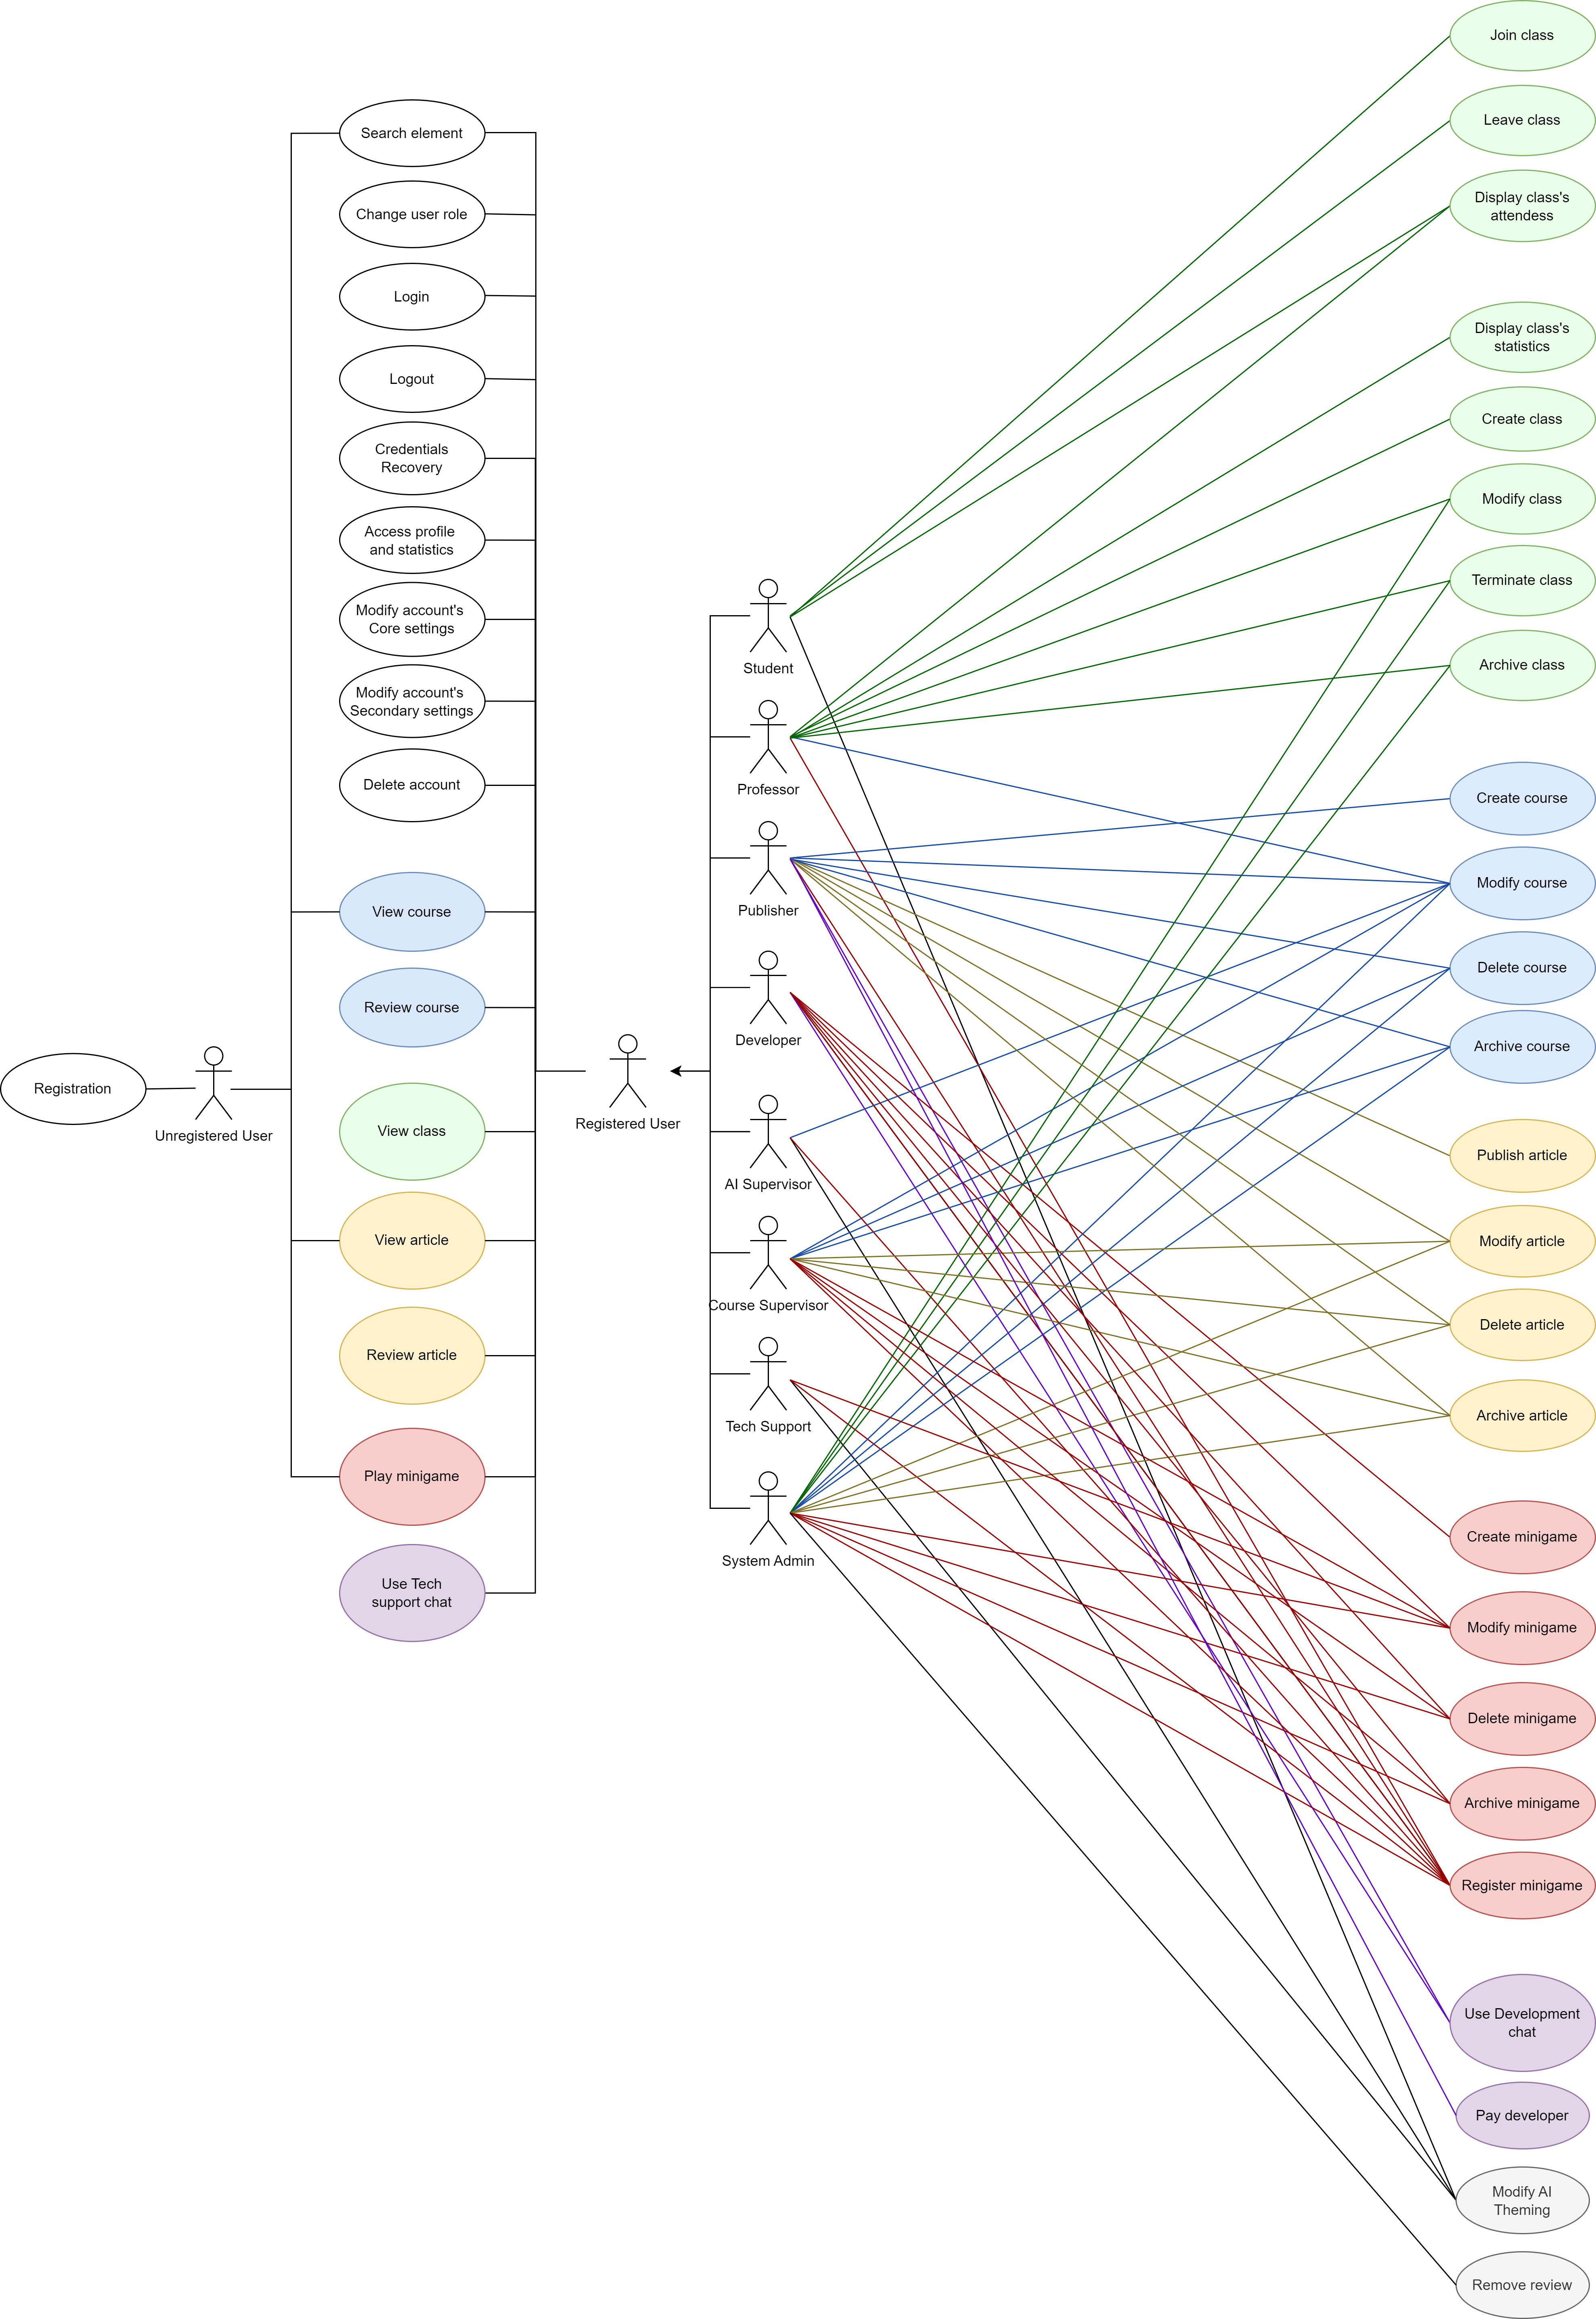
\includegraphics[width=0.9\textwidth]{images/usecase-diagram.png}
	\caption{Complete use case diagram}
	\label{fig:usecase-diagram}
\end{figure}

\newpage
\subsubsection{Account and general purpose}
\begin{figure}[h]
	\centering
	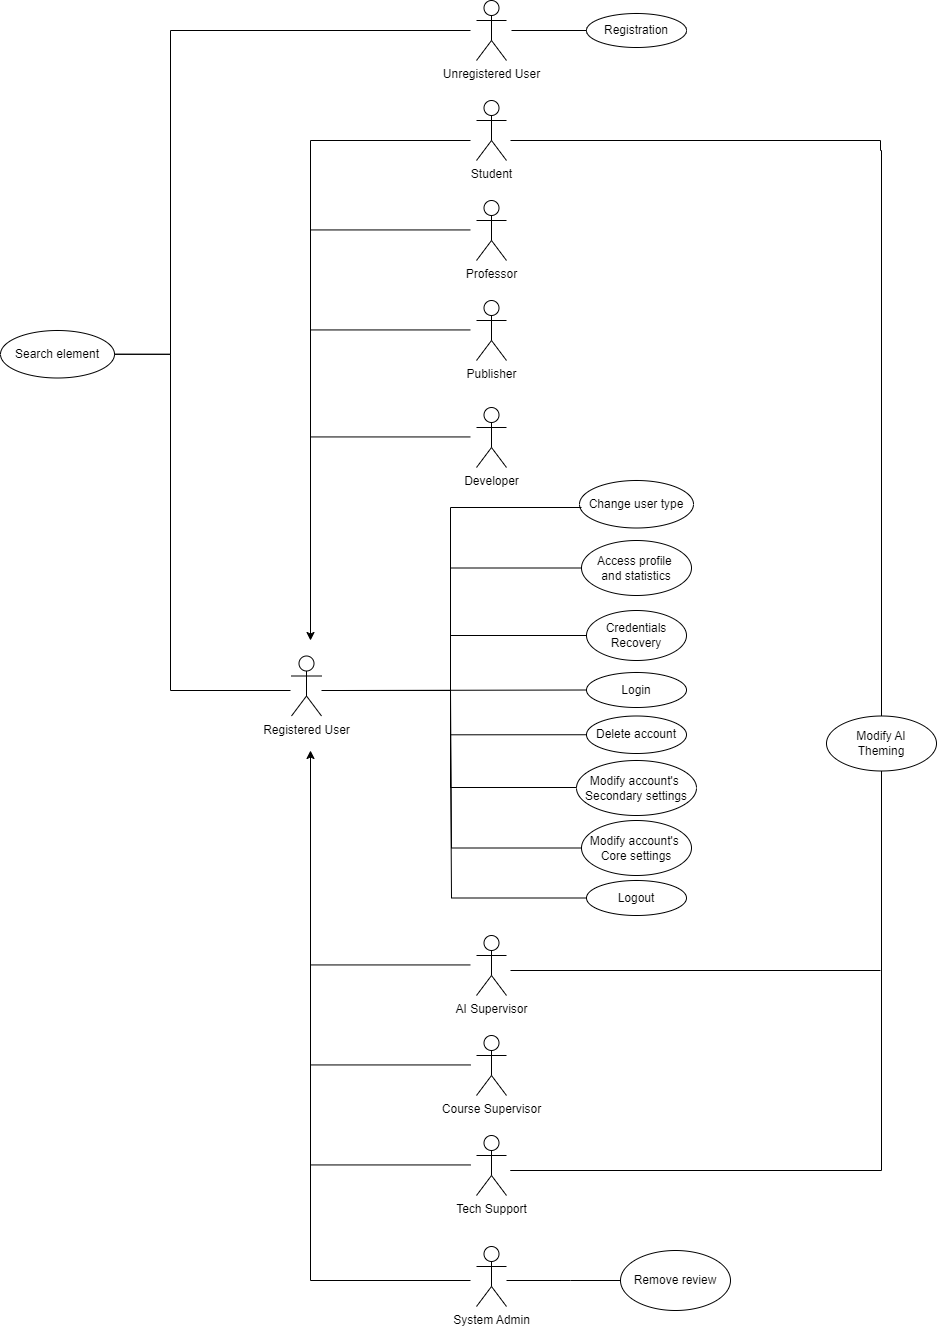
\includegraphics[width=0.7\textwidth]{images/UC-account.png}
	\caption{Use case diagram for account system}
	\label{fig:UC-account}
\end{figure}

\newpage
\subsubsection{Article}
\begin{figure}[h]
	\centering
	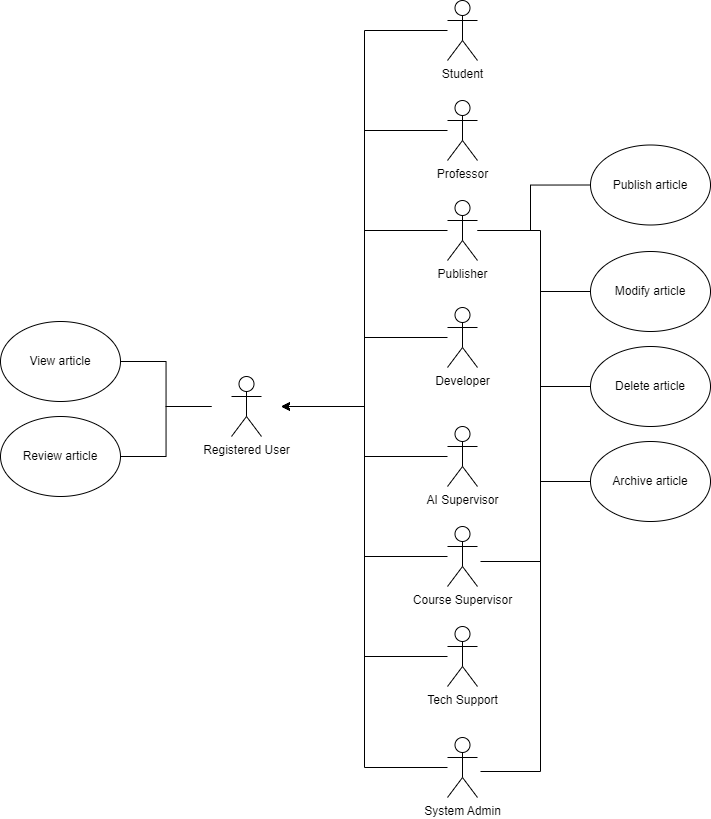
\includegraphics[width=0.9\textwidth]{images/UC-article.png}
	\caption{Use case diagram for article system}
	\label{fig:UC-article}
\end{figure}

\newpage
\subsubsection{Chat}
\begin{figure}[h]
	\centering
	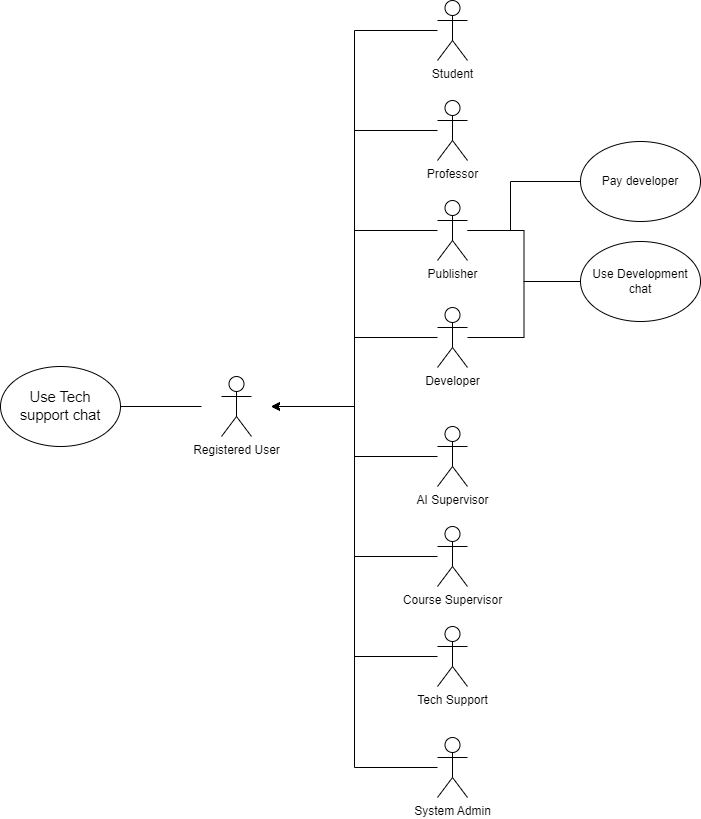
\includegraphics[width=0.9\textwidth]{images/UC-chat.png}
	\caption{Use case diagram for chat system}
	\label{fig:UC-chat}
\end{figure}

\newpage
\subsubsection{Class}
\begin{figure}[h]
	\centering
	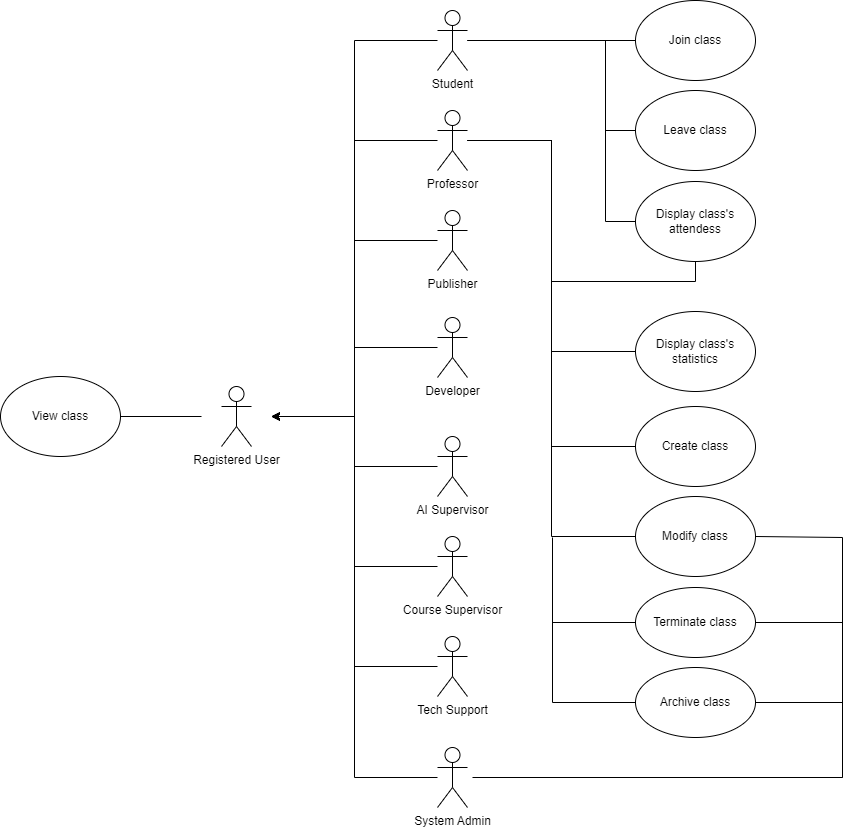
\includegraphics[width=0.9\textwidth]{images/UC-class.png}
	\caption{Use case diagram for class system}
	\label{fig:UC-class}
\end{figure}

\newpage
\subsubsection{Course}
\begin{figure}[h]
	\centering
	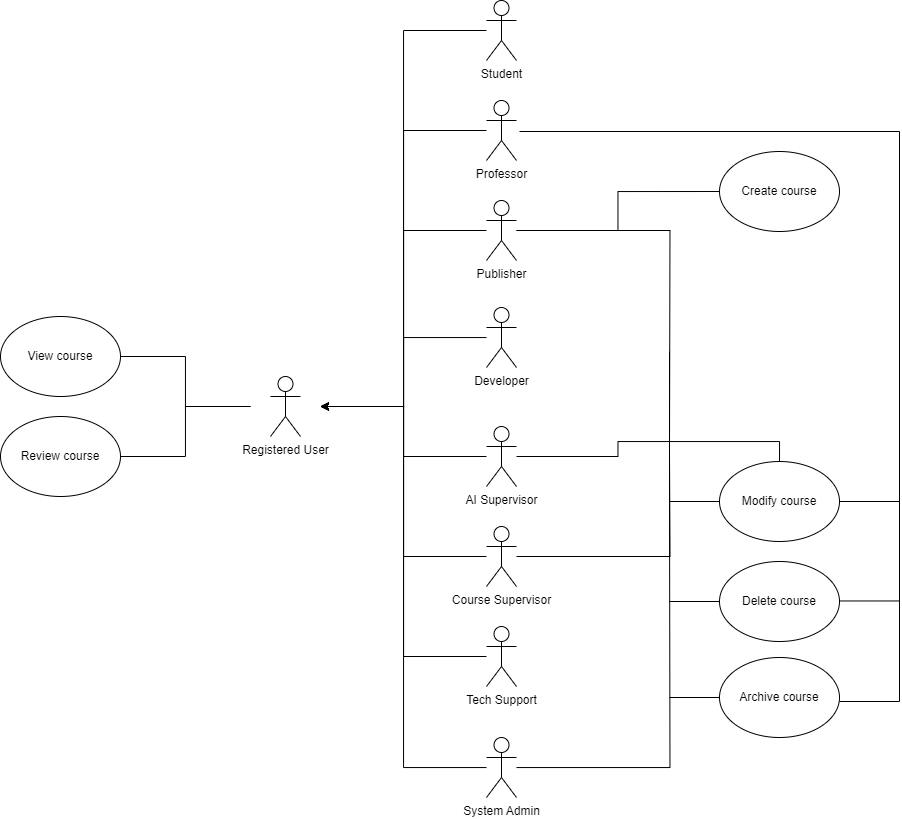
\includegraphics[width=0.9\textwidth]{images/UC-course.png}
	\caption{Use case diagram for course system}
	\label{fig:UC-course}
\end{figure}

\newpage
\subsubsection{Minigame}
\begin{figure}[h]
	\centering
	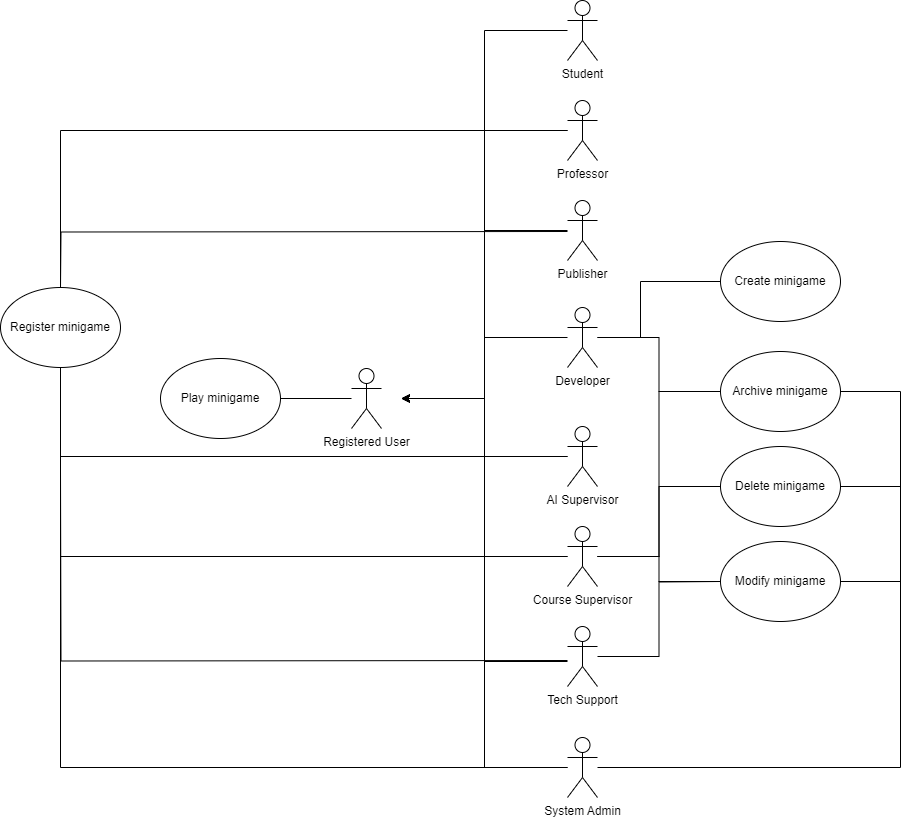
\includegraphics[width=0.9\textwidth]{images/UC-minigame.png}
	\caption{Use case diagram for minigame system}
	\label{fig:UC-course}
\end{figure}

	\newpage
	\section{Context Diagram} \label{context-diagram}
We created a context diagram separating the general roles (registered and unregistered users), the specific roles (all the others), the subsystems (payment, authentication, credential recovery, LLM) and the peer system (database).

\begin{figure}[h]
	\centering
	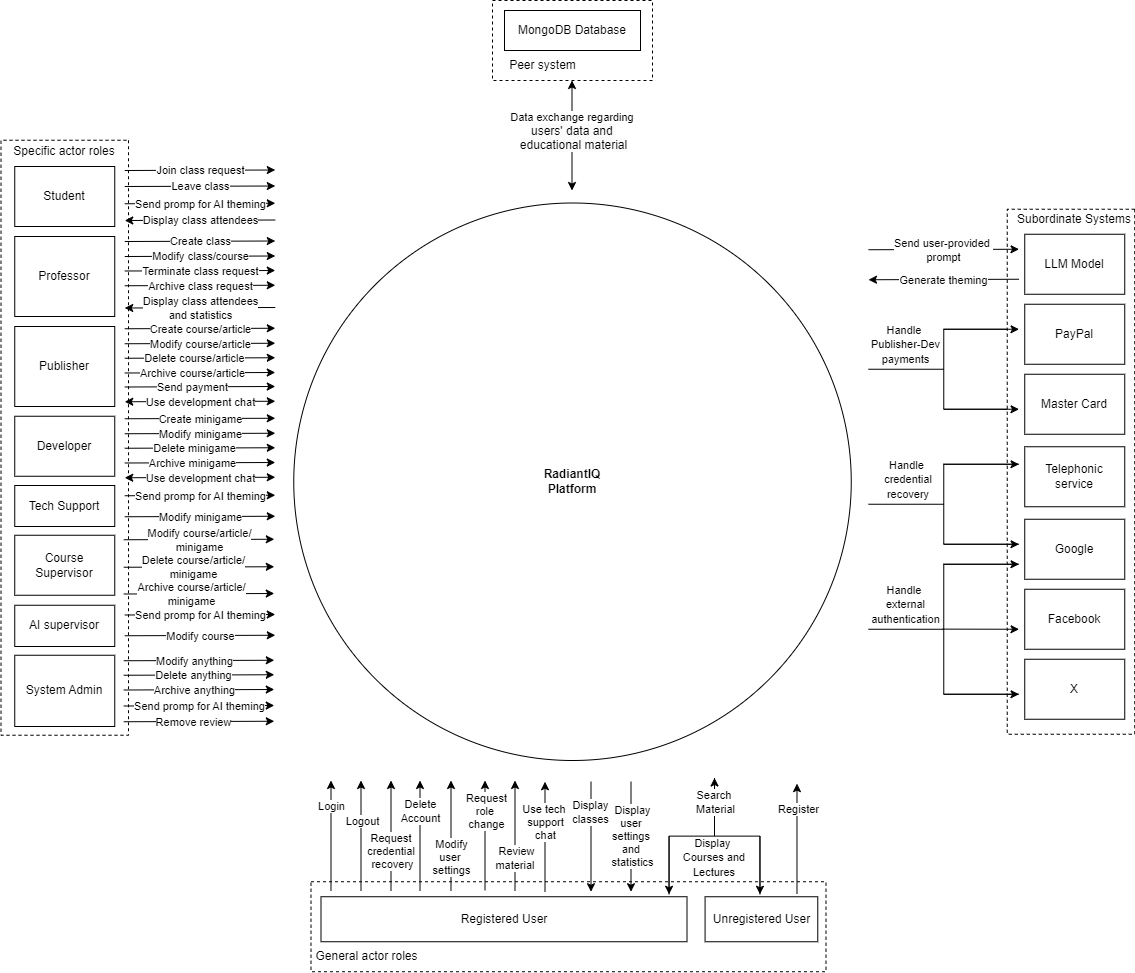
\includegraphics[width=1.0\textwidth]{images/ContextDiagram.png}
\end{figure}
	\newpage
	\section{Component Diagram} \label{component-diagram}


	\newpage
	\section{Class Diagram} \label{class-diagram}

The class diagram below in the UML describes the structure of RadianIQ's system by showing the main classes, their attributes, operations and their relationships.

\begin{figure}[H]
	\centering
	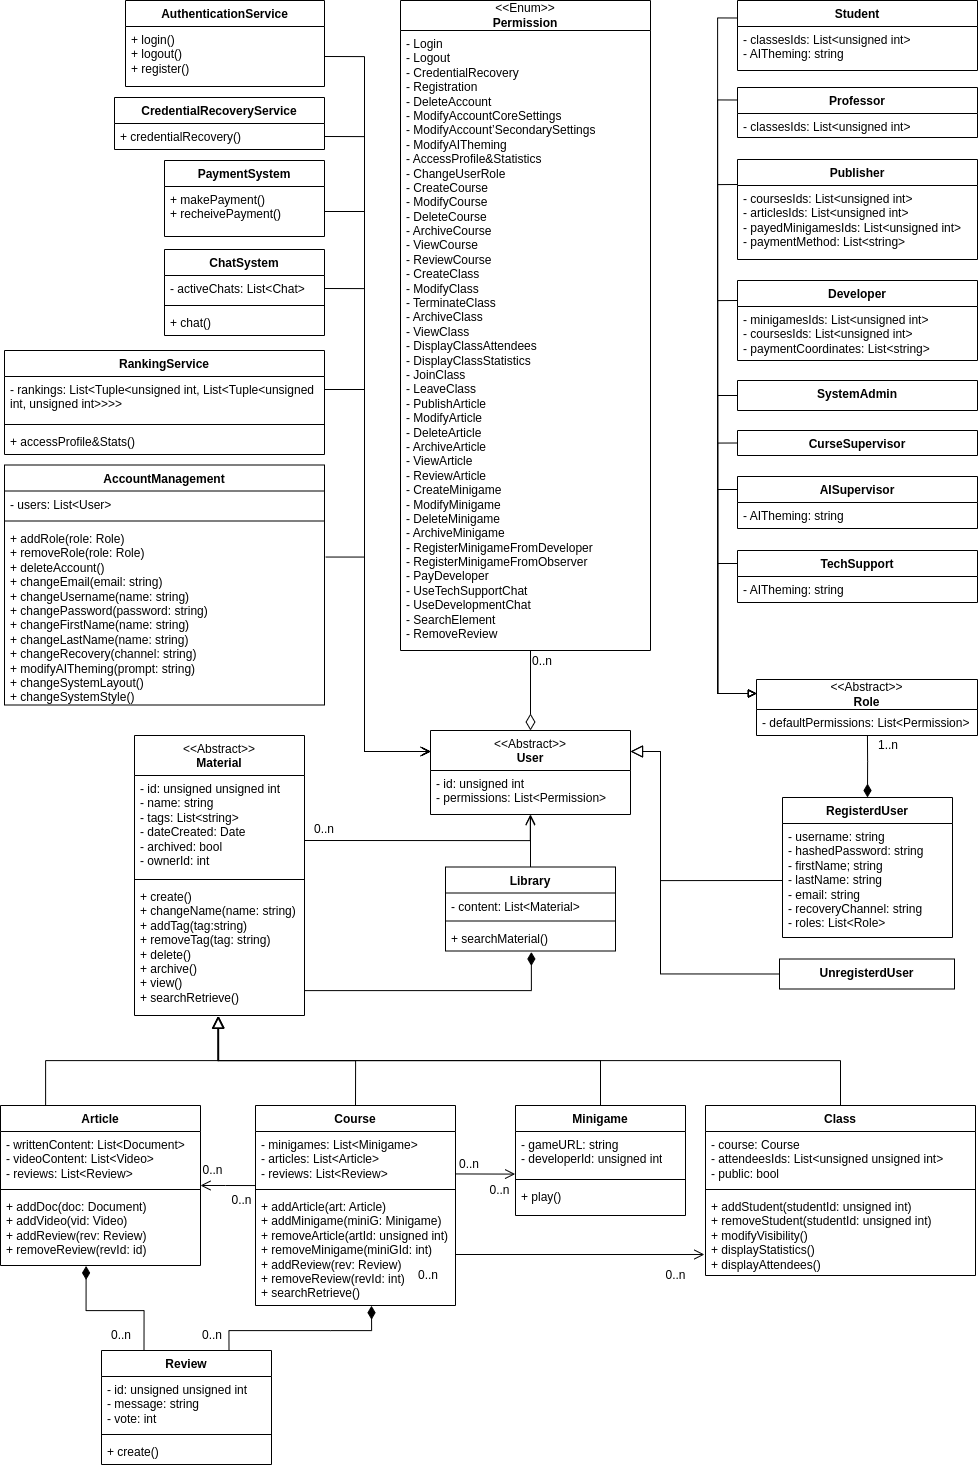
\includegraphics[width=0.85\linewidth]{images/class-diagram.png}
	\caption{RadiantIQ - Class diagram}
	\label{fig:class-diagram}
\end{figure}
	\newpage
	\section{Conclusion} \label{conclusion}


		
	\newpage
	
\end{document}
